\section{Applications} \label{apps}
In this section, uncertain design problems are transformed into robust programs to demonstrate and compare the methods above. The first problem (a simple aircraft model) is used mostly to clarify the concept, while the second (a large-scale solar-aicraft design code) shows the effectiveness of the tractable robust GP-approximation methods proposed.

\subsection{Simple Flight Design}
RGP formulation ideas were implemented on a simple wing design adapted from Hoburg \cite{hoburg_abbeel_2014}.

\begin{equation}
\begin{aligned}
	&\min &&D\\
	& s.t. &&C_D \geq \frac{C_{DA0}}{S} + kC_fS_{wet} + \frac{C_L^2}{\pi Ae}\\
	& &&W_W \geq W_{W_2} S + \frac{W_{W_1}N_{utl}A^{1.5}\sqrt{W_0WS}}{\tau}\\
	& &&D \geq 0.5\rho SC_DV^2\\
	& &&Re \leq \frac{\rho}{\mu}V\sqrt{\frac{S}{A}}\\
	& &&C_f \geq \frac{0.074}{Re^0.2}\\
	& &&W \leq 0.5\rho S C_LV^2\\
	& &&W \leq 0.5\rho S C_{Lmax}V_{min}^2\\
	& &&W \geq W_0 + W_W
\end{aligned}
\label{simple_wing}
\end{equation}
\ \\
This 8-constraint problem has two design variables ($A, S$), seven dependent free variables ($C_D, C_L, C_f, Re, W, W_W, V$), and the thirteen uncertain parameters in Table \ref{uncertain_simple_wing}. Note that the uncertainties specified in the table are the principal-axis widths of either the box or elliptical uncertainty sets. Note that uncertainties in this problem are only in the coefficients, and that constraints in \eqref{simple_wing} are predominantly monomials and two-term posynomials, with only one posynomial of more than two terms.

The problem is first solved for different sizes ($\Gamma$ values) of box and elliptical uncertainty sets (defined in Appendix \ref{LP_to_GP}), where the number of piecewise-linear terms is chosen such that the relative error between the solution of the upper tractable approximation and that of the lower tractable approximation is less than $0.1\%$. The design variables are then fixed for each solution so that the design can be simulated for 1000 realizations of the uncertain parameters to examine average design performance.

\begin{center}
\begin{tabular}{ |P{7em}|P{3.5cm}|P{5.2cm}|}
\hline
Uncertain Parameter & Value & Description \\
\hline
$C_{DA0}$ & $0.035 \pm 42.85\%$ $[m^2]$ & Fuselage Drag Area\\
\hline
$k$ & $1.17 \pm 31.11\%$ & Form Factor \\
\hline
$S_{wet}$ & $2.075 \pm 3.61\%$ & Wetted Area Ratio\\  
\hline
$e$ & $0.92 \pm 7.60$ & Oswald Efficiency Factor\\  
\hline
$W_{W_2}$ & $60 \pm 66\%$ $[Pa]$ & Wing Weight Coefficient 2\\  
\hline
$W_{W_1}$ & $12e^{-5} \pm 60\%$ $[\frac{1}{m}]$ & Wing Weight Coefficient 1\\  
\hline
$N_{utl}$ & $3.3 \pm 33.33\%$ & Ultimate Load Factor\\  
\hline
$W_0$ & $6250 \pm 60\%$ $[N]$ & Aircraft Weight Excluding Wing\\  
\hline
$\tau$ & $0.12 \pm 33.33\%$ & Airfoil Thickness to Chord Ratio\\  
\hline
$\rho$ & $1.23 \pm 10\%$ $[\frac{kg}{m^3}]$ & Density of Air\\  
\hline
$\mu$ & $1.775e^{-5} \pm 4.22\%$ $[\frac{kg}{ms}]$ & Viscosity of Air\\  
\hline
$C_{Lmax}$ & $1.6 \pm 25\%$ & Maximum Lift coefficient of Wing\\  
\hline
$V_{min}$ & $25 \pm 20\%$ $[\frac{m}{s}]$ & Takeoff Speed\\  
\hline
\end{tabular}
\captionof{table}{Uncertain parameters in the simple wing design.}
\label{uncertain_simple_wing}
\end{center}

We can see from Figure \ref{simple_wing_var_gamma} that while probability of failure goes to zero as $\Gamma$ increases. Descriptions of how $\Gamma$ determines the size of uncertainty sets are in Appendices \ref{box_linear_app} and \ref{ellip}. For a given level of risk, the average performance of designs robust to an elliptical uncertainty set is better than that of those using a box uncertainty set.

% TODO: ALI same y axis scale?
\begin{figure}[h]
    \centering
    \captionsetup{justification=centering, font=small}
    \begin{subfigure}{0.49\textwidth}
        \centering
        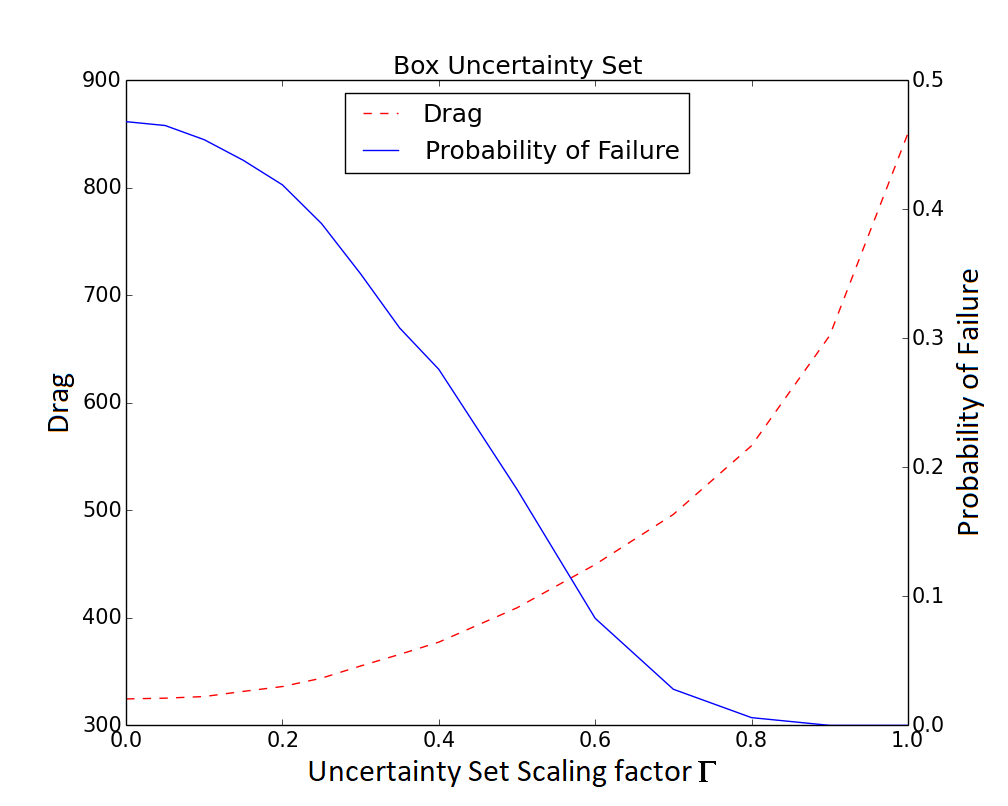
\includegraphics[height=1.85in]{simple_wing_results/box.png}
        % \caption{Box Uncertainty Set Objective Value}
    \end{subfigure}%
    ~ 
    \begin{subfigure}{0.49\textwidth}
        \centering
        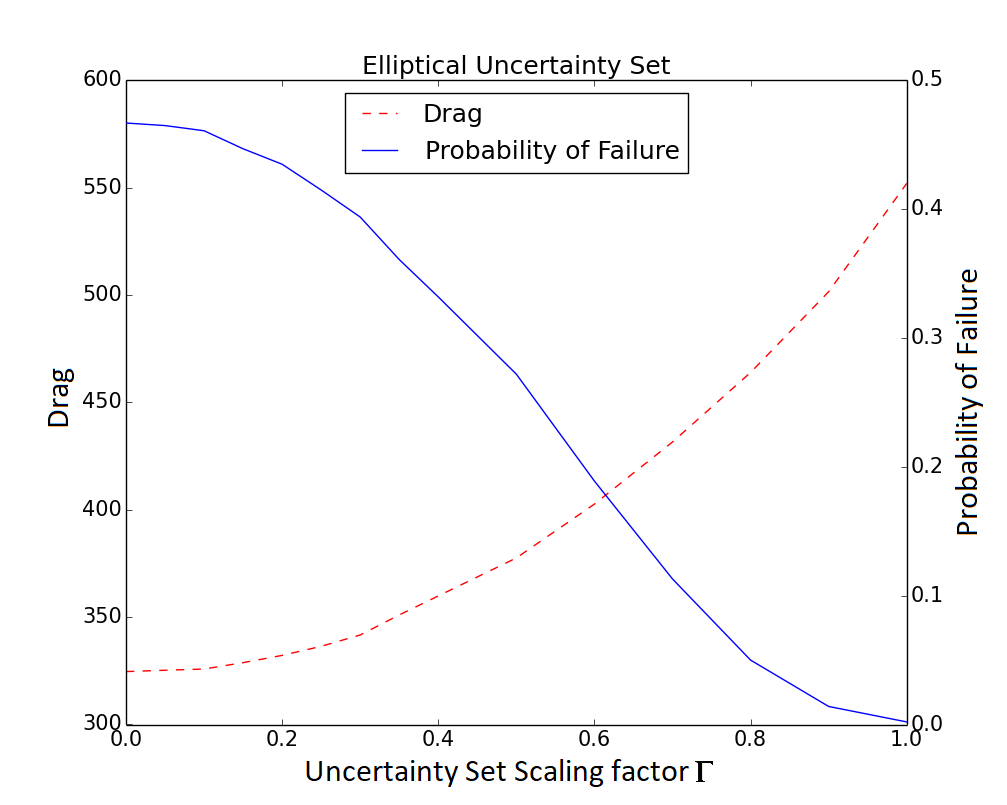
\includegraphics[height=1.85in]{simple_wing_results/ell.png}
        % \caption{Box Uncertainty Set Probability of Failure}
    \end{subfigure}
    \caption{Performance of the optimal robust simple wing, using the Best Pairs formulation, as a function of $\Gamma$ for different uncertainty sets.}
    \label{simple_wing_var_gamma}
\end{figure}

Table \ref{simp_table} and Figure \ref{compare_simple_wing} compare the results of robustifying and solving the simple wing design problem with different methodologies. The number of piecewise-linear terms per two-term posynomial needed to reach a $0.1\%$ tolerance is much higher for the Two Term formulation from \cite{hsiung_kim_boyd_2007} than for our formulations. Correspondingly, the total number of constraints needed by the two-term formulation is also much larger.

\begin{center}
\begin{tabular}{ |m{7em}|m{1.8cm}|m{1.5cm}|m{2.2cm}|m{1.8cm}| }
\hline
Method & Uncertainty Set & Relative Error [$\%$] & Number of PWL Sections & Number of Constraints \\
\hline
\multirow{2}{7em}{Two Term} & Box & 0.1 & 79 & 327\\ 
& Elliptical & 0.1 & 70 & 291\\
\hline
\multirow{2}{7em}{Simple Conservative} & Box & 0 & 0 & 16\\ 
& Elliptical & 0 & 0 & 16 \\
\hline
\multirow{2}{7em}{Linearized Perturbations} & Box & 0 & 0 & 16\\ 
& Elliptical & 0.1 & 31 & 49 \\  
\hline
\multirow{2}{7em}{Best Pairs} & Box & 0 & 0 & 16\\ 
& Elliptical & 0.1 & 40 & 93 \\
\hline
Deterministic & N/A & N/A & N/A & 8\\
\hline
\end{tabular}
\captionof{table}{Simple wing results}
\label{simp_table}
\end{center}

Our methodologies achieved an exact solution for the box uncertainty set as condition $C_3$ (Section \ref{Conservative}) is satisfied, and therefore no piecewise-linearization is needed. This explains the identical results of our three methodologies for the box uncertainty set in Figures \ref{compare_simple_wing} and \ref{simple_wing_var_pwl}, constrasting with the more than 70 piecewise-linear sections needed by the two-term formulation to achieve a $0.1\%$ tolerance. Condition $C_3$ is not satisfied for the elliptical uncertainty set, and so here our simple method is noticeably more conservative than those using piecewise-linear approximations.

\begin{figure}[h]
    \centering
    \captionsetup{justification=centering, font=small}
    \begin{subfigure}{0.49\textwidth}
        \centering
        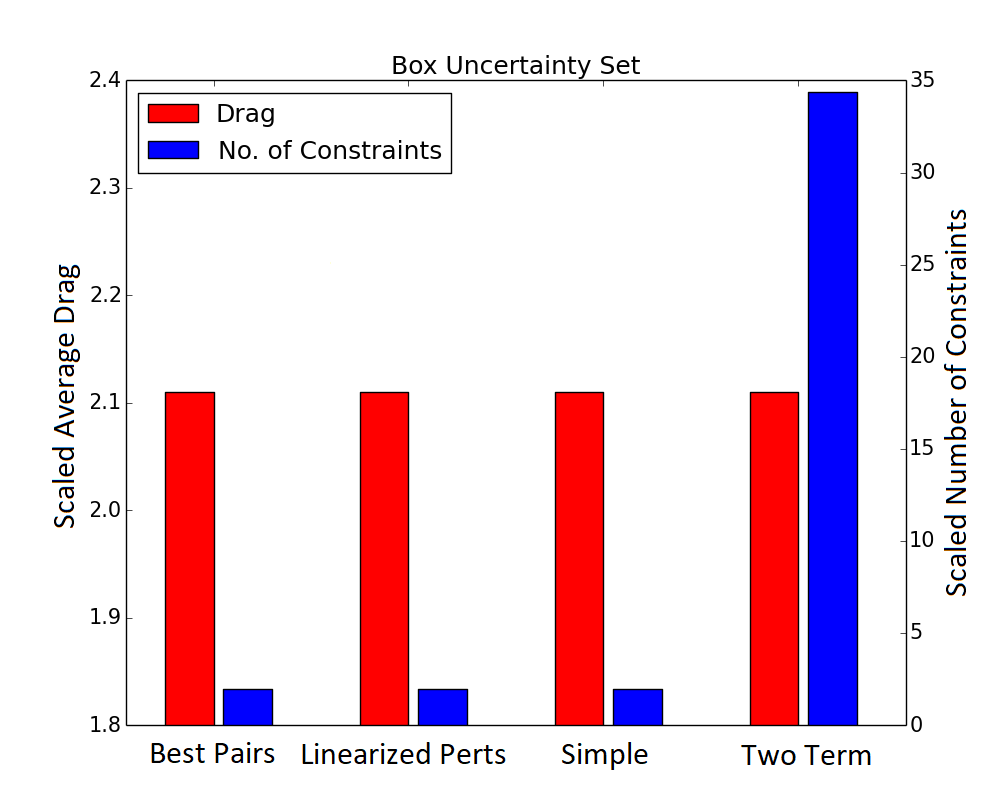
\includegraphics[height=1.85in]{simple_wing_results/box_obj_cons.png}
        % \caption{Box Uncertainty Set Objective Value}
    \end{subfigure}%
    ~ 
    \begin{subfigure}{0.49\textwidth}
        \centering
        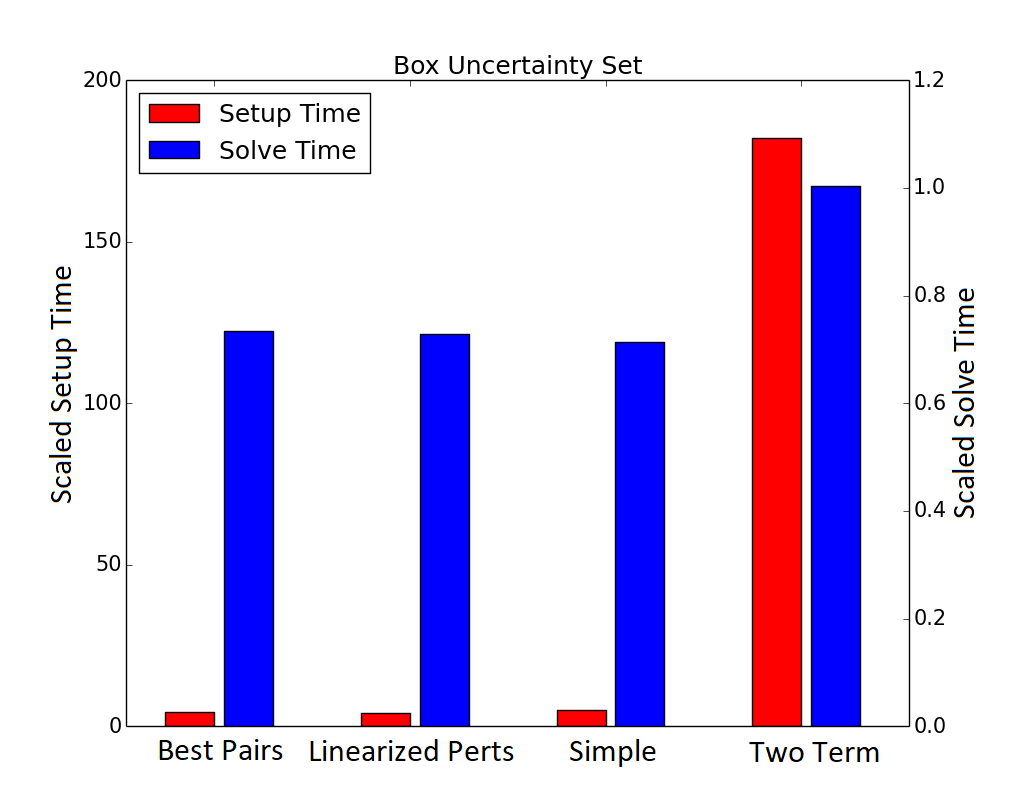
\includegraphics[height=1.85in]{simple_wing_results/box_times.png}
        % \caption{Box Uncertainty Set Probability of Failure}
    \end{subfigure}
    ~
    \begin{subfigure}{0.49\textwidth}
        \centering
        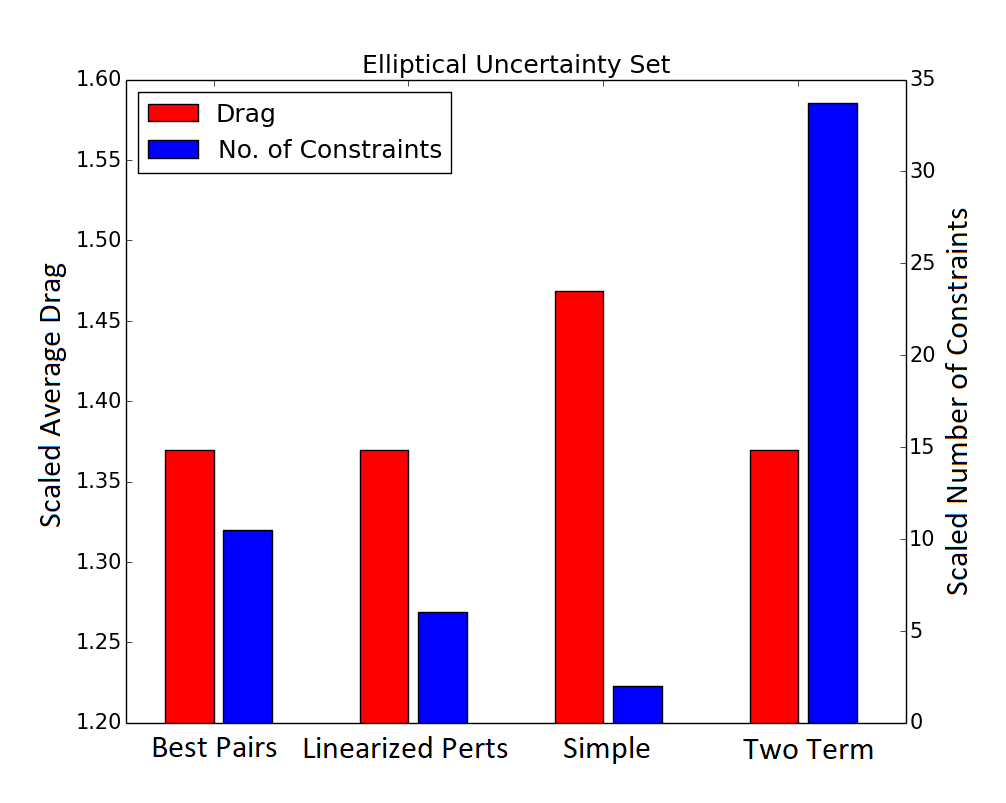
\includegraphics[height=1.85in]{simple_wing_results/ell_obj_cons.png}
        % \caption{Elliptical Uncertainty Set Objective Value}
    \end{subfigure}%
    ~ 
    \begin{subfigure}{0.49\textwidth}
        \centering
        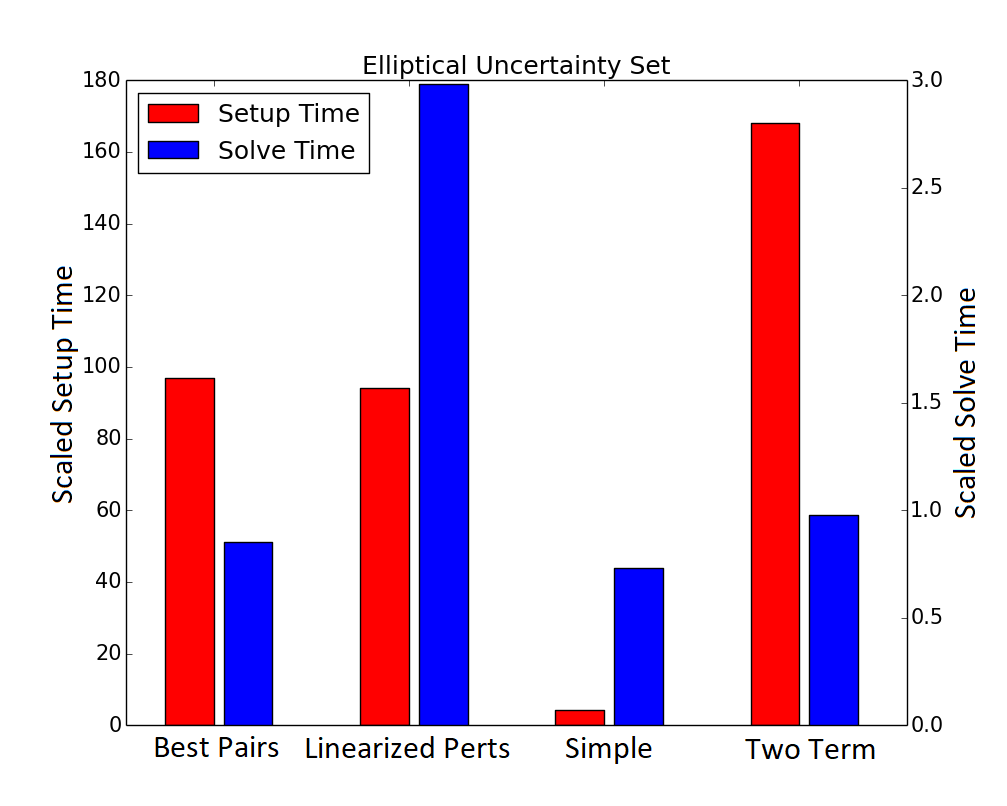
\includegraphics[height=1.85in]{simple_wing_results/ell_times.png}
        % \caption{Elliptical Uncertainty Set Probability of Failure}
    \end{subfigure}
    \caption{Robust simple wing design results relative to the nomial design problem.}
    \label{compare_simple_wing}
\end{figure}

\begin{figure}[H]
    \centering
    \captionsetup{justification=centering, font=small}
    \begin{subfigure}{0.49\textwidth}
        \centering
        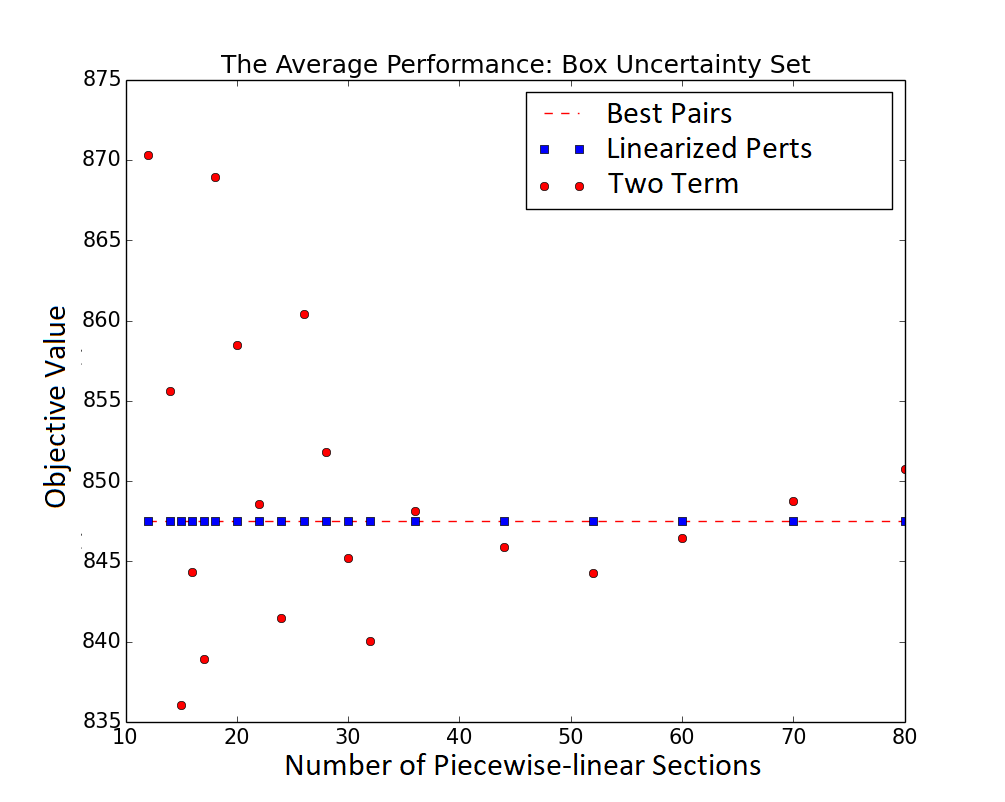
\includegraphics[height=1.85in]{simple_wing_results/box_avg_pwl.png}
        % \caption{Box Uncertainty Set Objective Value}
    \end{subfigure}%
    \begin{subfigure}{0.49\textwidth}
        \centering
        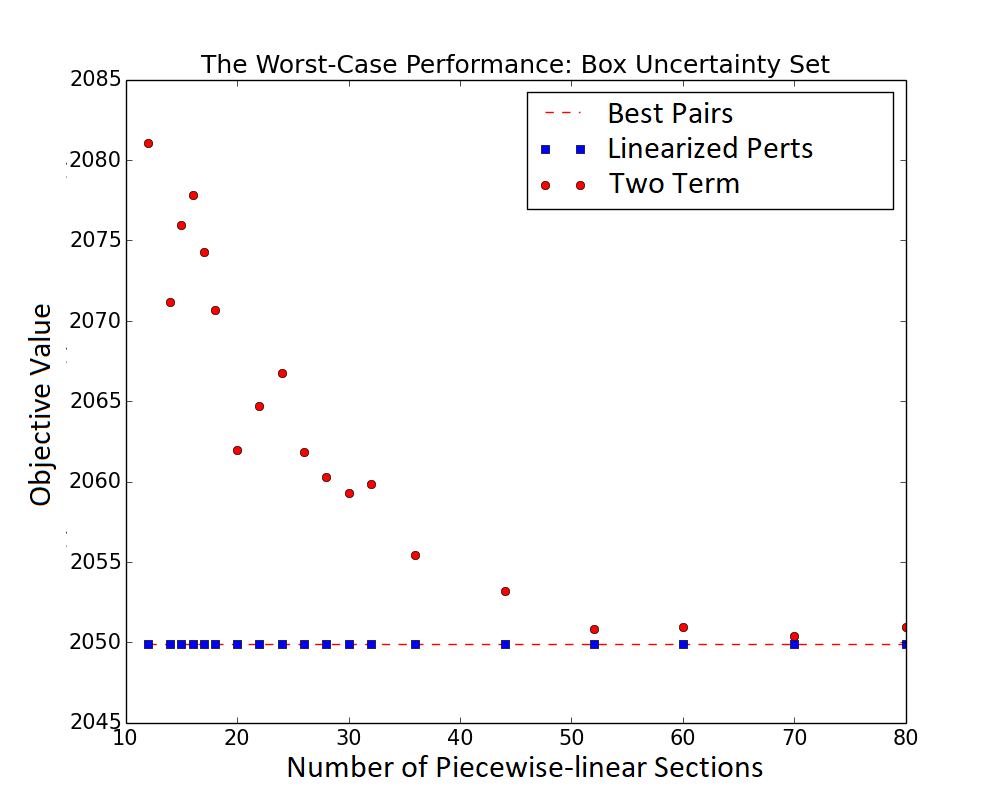
\includegraphics[height=1.85in]{simple_wing_results/box_worst_pwl.png}
        % \caption{Box Uncertainty Set Probability of Failure}
    \end{subfigure}
    \begin{subfigure}{0.49\textwidth}
        \centering
        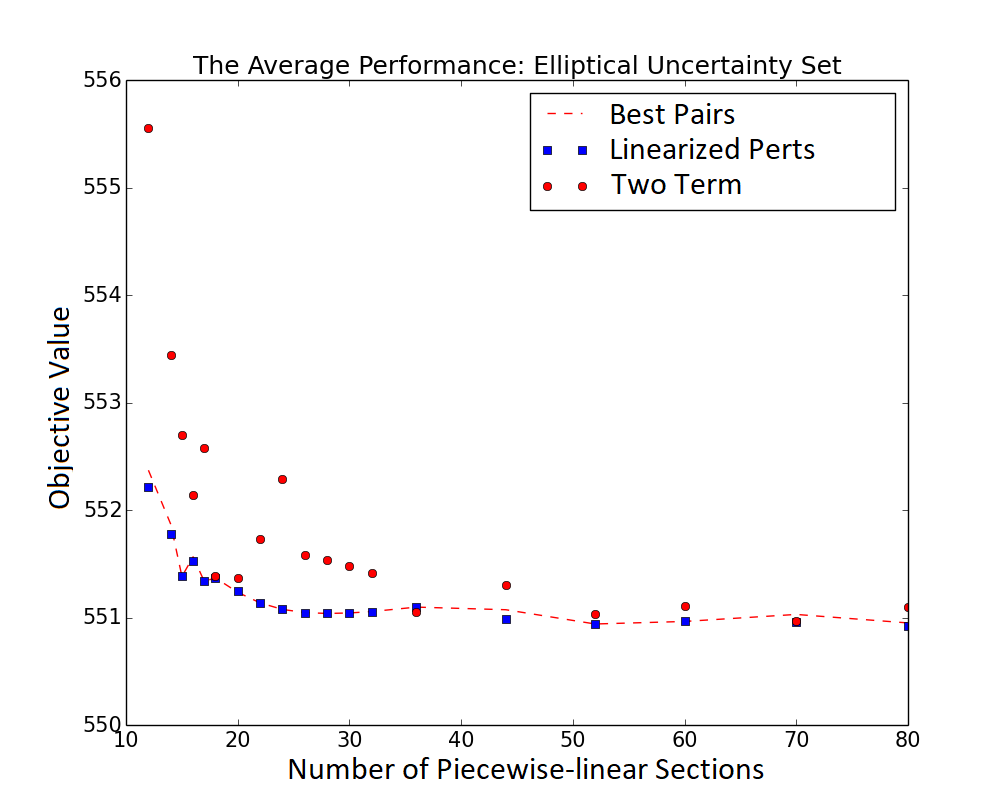
\includegraphics[height=1.85in]{simple_wing_results/ell_avg_pwl.png}
        % \caption{Elliptical Uncertainty Set Objective Value}
    \end{subfigure}%
    \begin{subfigure}{0.49\textwidth}
        \centering
        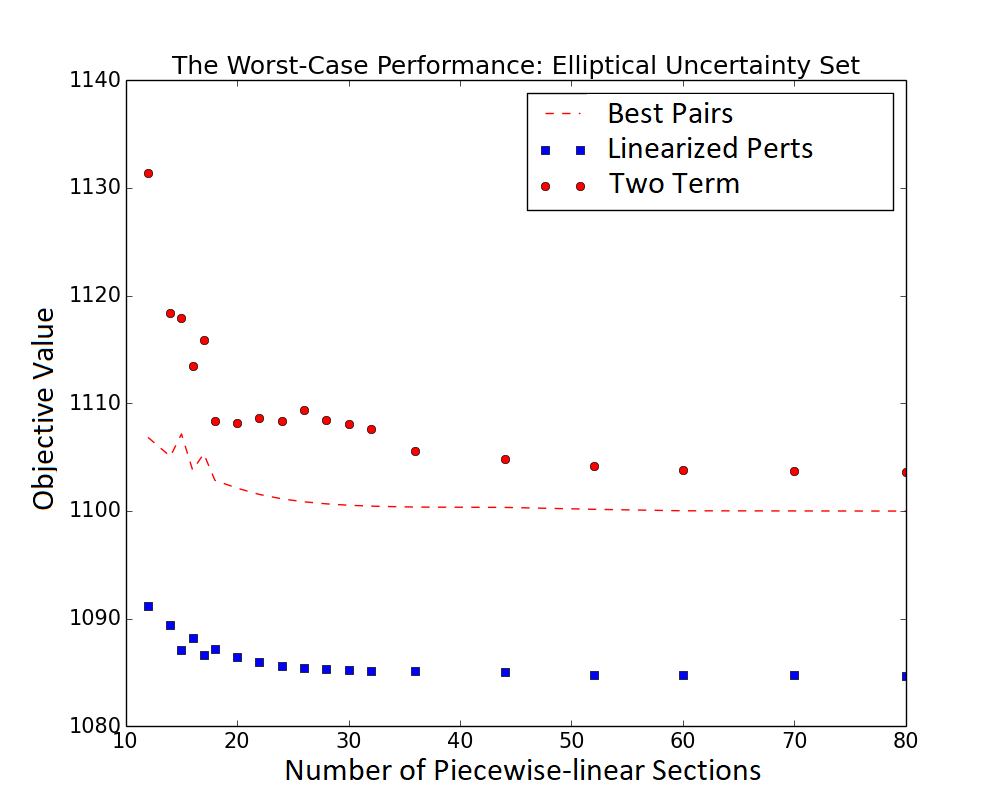
\includegraphics[height=1.85in]{simple_wing_results/ell_worst_pwl.png}
        % \caption{Elliptical Uncertainty Set Probability of Failure}
    \end{subfigure}
    \caption{The performance (objective value) of the simple wing design as a function of the number of piecewise-linear terms}  % TODO caption could use some work
    \label{simple_wing_var_pwl}
\end{figure}


\subsection{UAV Solar Model}
In previous GP modeling work, Burton presented a GP-compatible solar-powered aircraft model \cite{burton_hoburg} designed to fulfill the requirements in Table \ref{mission_requirement}. The nominal model is formed of 2698 constraints including 20 design variables, 875 dependent free variables, and 271 uncertain parameters. Table \ref{uncertain_solar} presents a sample of the uncertain parameters in the solar aircraft design.\\

\begin{table}[ht]
\begin{minipage}[b]{0.38\linewidth}
\centering
\begin{tabu}{P{6em}|P{1.9cm}}
    \tabucline[1pt]{1-6}
    \multicolumn{2}{c}{\textbf{Mission Requirements}} \\ \tabucline[1pt]{1-6}
    Payload & $10$ $lbs$ \\ \hline
    Station Keeping & $90\%$ $winds$\\ \hline
    Endurance & $> 5$ $days$\\ \hline
    Season & $all$ $seasons$\\ \hline
    Altitude & $> 4600$ $m$\\ \hline
    Latitude & $\pm 30^\circ$\\ \hline
   \end{tabu}
    \caption{Mission requirements.}
    \label{mission_requirement}
\end{minipage}\hfill
\begin{minipage}[b]{0.62\linewidth}
\centering
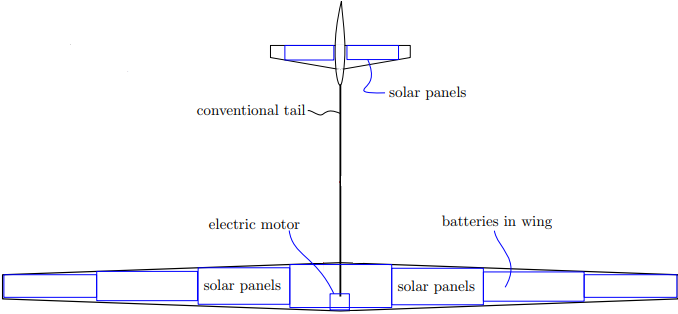
\includegraphics[width=80mm]{solar_results/solarAircraft.PNG}
\captionof{figure}{Solar aircraft planform.}
\label{the_aircraft}
\end{minipage}
\end{table}


\begin{center}
\begin{tabular}{ |P{10em}|P{3cm}|P{4cm}|}
\hline
Uncertain Parameter & Value & Description \\
\hline
$\eta_m$ & $0.95 \pm 7\%$ & Motor Efficiency\\
\hline
$h_{batt}$ & $350 \pm 15\%$ $[\frac{Wh}{Kg}]$ & Battery Specific Energy \\
\hline
$\eta_{solar}$ & $0.22 \pm 15\%$ & Solar Cell Efficiency\\
\hline
$V_{wind_{ref}}$ & $100 \pm 3\%$ $[\frac{m}{s}]$ & Reference Wind Speed\\  
\hline
$\eta_{prop}$ & $0.8 \pm 10\%$ & Propeller Efficiency\\
\hline
\end{tabular}
\captionof{table}{A sample of the solar aircraft uncertain parameters}
\label{uncertain_solar}
\end{center}

This problem was solved for an elliptical uncertainty set for various values of $\Gamma$ with a maximum number of piecewise-linear terms of 50 and a desired relative error of 1\% between the solution of the upper and lower tractable approximations. The average performance was then calculated from 300 realizations.

Table \ref{solar_table} and Figure \ref{compare_solar} show that the number of constraints needed to formulate this approximate RGP with the Two Term formulation is extremely large even at a relative error of 2\%. By comparison, the formulations presented in this paper have a relatively small number of constraints, primarily due to the partitioning of large posynomials into smaller ones.

\begin{center}
\begin{tabular}{ |m{7em}|m{1.8cm}|m{1.5cm}|m{2.2cm}|m{1.8cm}| }
\hline
Method & Uncertainty Set & Relative Error [$\%$] & Number of PWL Sections & Number of Constraints \\
\hline
\multirow{2}{7em}{Two Term} & Box & 2.3 & 50 & 91,599\\ 
& Elliptical & 2.2 & 50 & 91,599\\
\hline
\multirow{2}{7em}{Simple Conservative} & Box & 0 & 0 & 2,896\\ 
& Elliptical & 0 & 0 & 2,896 \\
\hline
\multirow{2}{7em}{Linearized Perturbations} & Box & 0 & 0 & 3,895\\ 
& Elliptical & 0.9 & 31 & 2,899 \\  
\hline
\multirow{2}{7em}{Best Pairs} & Box & 0.7 & 4 & 2,939\\ 
& Elliptical & 0.9 & 32 & 4,433 \\
\hline
Deterministic & N/A & N/A & N/A & 2,837\\
\hline
\end{tabular}
\captionof{table}{Solar aircraft results.}
\label{solar_table}
\end{center}

\begin{figure}[h]
    \centering
    \captionsetup{justification=centering, font=small}
    \begin{subfigure}{0.49\textwidth}
        \centering
        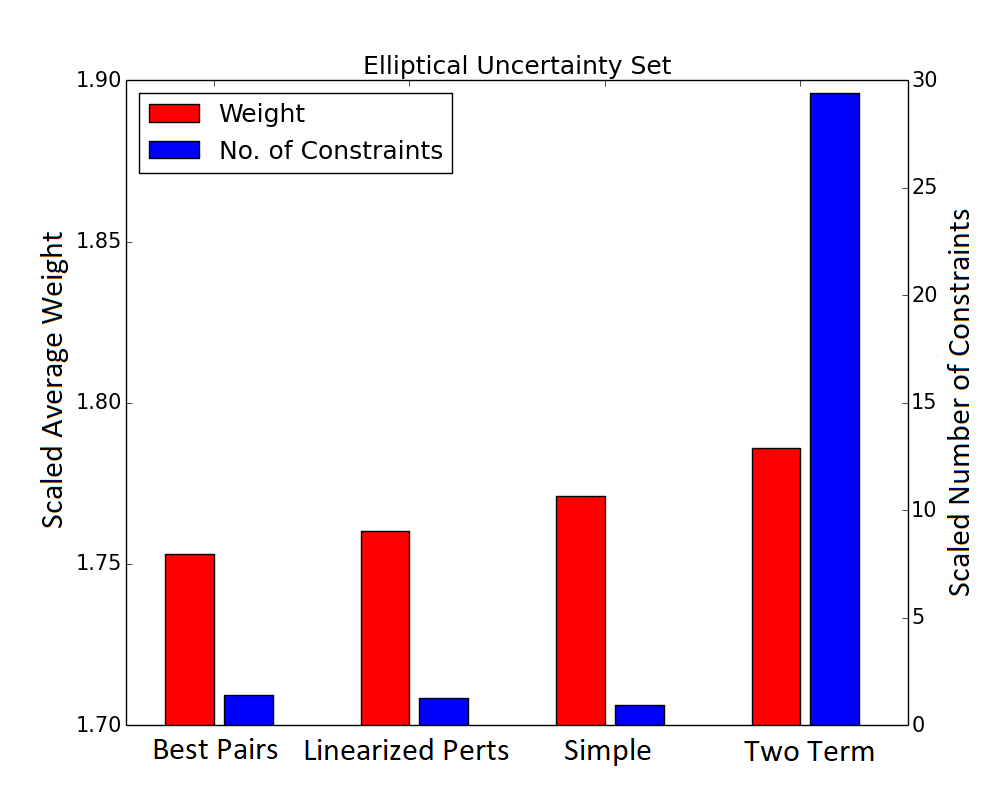
\includegraphics[height=1.85in]{solar_results/ell_obj_cons.png}
        % \caption{Elliptical Uncertainty Set Objective Value}
    \end{subfigure}%
    ~ 
    \begin{subfigure}{0.49\textwidth}
        \centering
        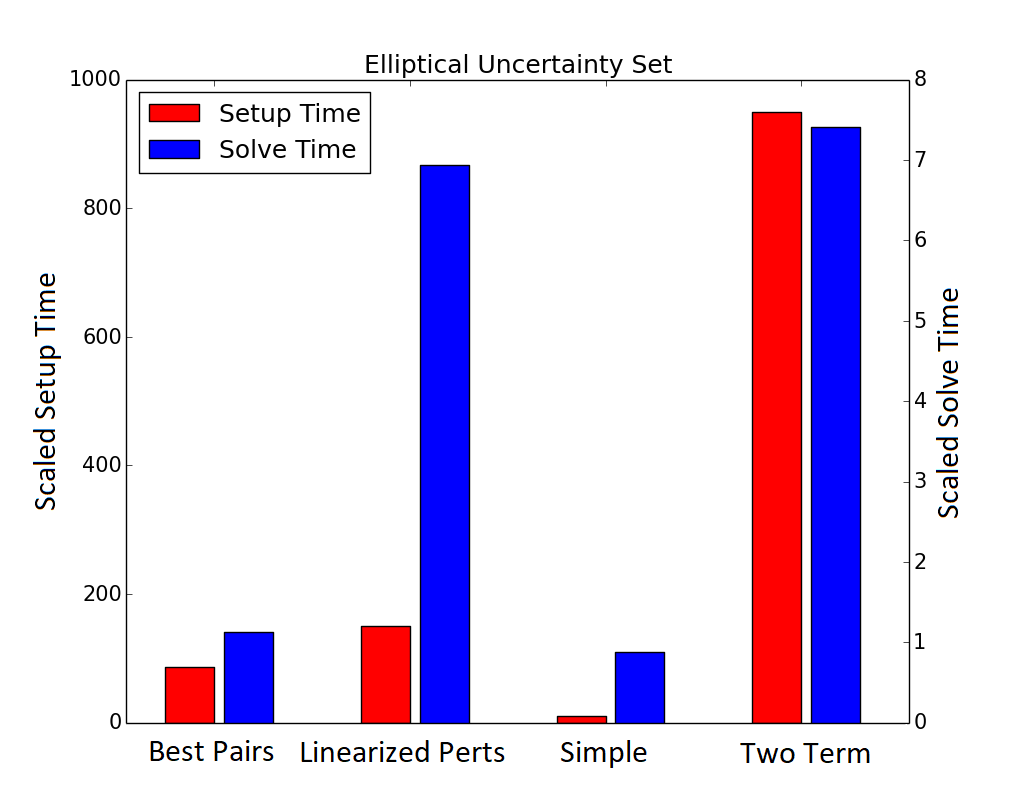
\includegraphics[height=1.85in]{solar_results/ell_time.png}
        % \caption{Elliptical Uncertainty Set Probability of Failure}
    \end{subfigure}
    \caption{Robust solar aircraft results scaled by nominal objective value, number of constraints, and timing.}
    \label{compare_solar}
\end{figure}

\begin{figure}
    \centering
    \captionsetup{justification=centering, font=small}
    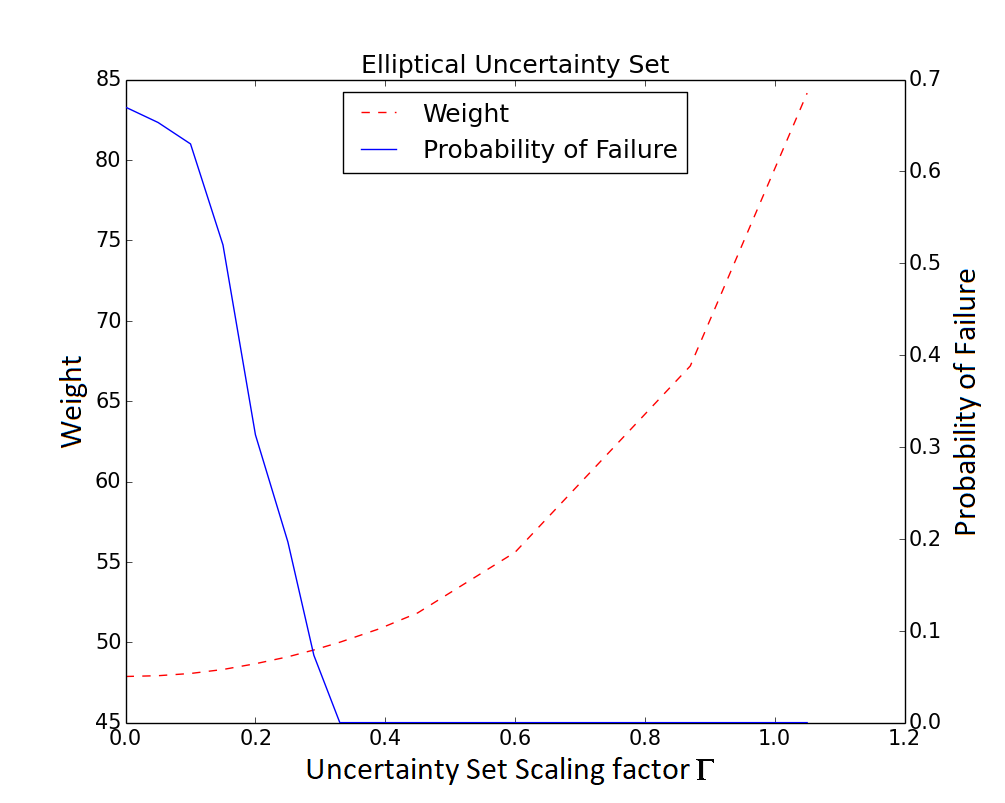
\includegraphics[height=3.5in]{solar_results/ell.png}
    \caption{Performance of the solar aircraft design based on the Best Pairs formulation, as a function of $\Gamma$.}
    \label{solar_var_gamma}
\end{figure}

Figure \ref{solar_var_gamma} shows that the probability of failure in the robust design goes to zero as $\Gamma$ increases, while the nominal design fails with a probability of 0.7.

\begin{figure}[h]
    \centering
    \captionsetup{justification=centering, font=small}
    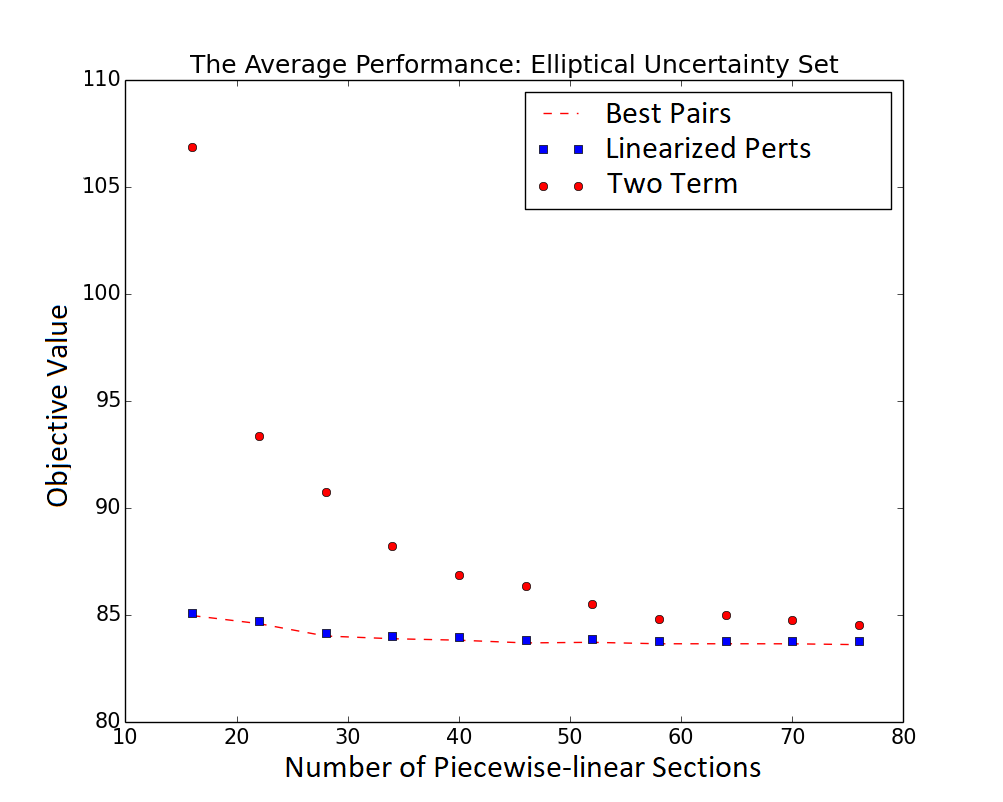
\includegraphics[scale=0.48]{solar_results/ell_avg_pwl.png}
    \caption{The performance of the solar aircraft design as a function of the number of piecewise-linear terms for elliptical uncertainty set}
    \label{solar_var_pwl}
\end{figure}
\begin{comment}
\end{comment}

As shown in Figure \ref{compare_solar}, the programs influenced by our formulations take much less time to  setup and solve than the Two Term formulation (with the exception of the the Linearized Perturbations solve), and all have better performance. Figure \ref{solar_var_pwl} additionally shows the fast convergence of the Best Pairs and Linearized Perturbations formulations with respect to the number of piecewise-linear terms used.